\documentclass[10pt, conference]{IEEEtran}
\usepackage{subimages}
\setfigdir{figs}
\usepackage[cmex10]{amsmath}
\interdisplaylinepenalty=2500

\usepackage{amsthm}
\newtheorem{definition}{Definition}

\usepackage{hyperref}

% correct bad hyphenation here
\hyphenation{op-tical net-works semi-conduc-tor}

\usepackage{todonotes}
\begin{document}
%
% paper title
% can use linebreaks \\ within to get better formatting as desired
\title{Real Time Eye Gaze Tracking Using Microsoft Kinect}

%------------------------------------------------------------------------- 
% change the % on next lines to produce the final camera-ready version 
\newif\iffinal
\finalfalse
% \finaltrue
\newcommand{\jemsid}{99999}
%------------------------------------------------------------------------- 

% author names and affiliations
% use a multiple column layout for up to two different
% affiliations

\iffinal
  \author{%
    \IEEEauthorblockN{Raul Benites Paradeda}
    \IEEEauthorblockA{%
      INESC-ID \& Instituto Superior T\'{e}cnico\\
      University of Lisbon\\
      Lisbon, Portugal\\
      Email: \href{mailto:raul.paradeda@tecnico.ulisboa.pt}{raul.paradeda@tecnico.ulisboa.pt}}
  \and
    \IEEEauthorblockN{Jones Granatyr, Jean Paul Barddal}
    \IEEEauthorblockA{%
      Graduate Program in Informatics (PPGIa)\\
      Pontif\'{i}cia Universidade Cat\'{o}lica do Paran\'{a} (PUCPR)\\
      Curitiba, Brazil\\
      Email:  \href{mailto:jones.granatyr@pucpr.edu.br}{jones.granatyr@pucpr.edu.br}, \href{mailto:jean.barddal@ppgia.pucpr.br}{jean.barddal@ppgia.pucpr.br}}
   \and
    \IEEEauthorblockN{Alberto Signoretti}
    \IEEEauthorblockA{%
      Graduate Program in Computer Science \\
      State Universtity of Rio Grande do Norte (UERN)\\
      Natal, Brazil\\
      Email:  \href{mailto:albertosignoretti@uern.br}{albertosignoretti@uern.br}}
  }
\else
  \author{Sibgrapi paper ID: \jemsid \\ }
\fi

% make the title area
\maketitle


\begin{abstract}
	This work presents a technique used to identify in real time, the focus region of the user's gaze through of a Kinect device, and how long the user’s focus is maintained over a specific region of the environment. The technique is divided in two stages. In the first one, the capture of the gaze is performed in two parts, the first one uses predefined regions, and the second is based on regions created using as criteria the user focus of the length of time on each part of the scenario. The second stage performs an algorithm of classification to identify the iris position. As a result, the technique showed that is possible identify and measure how long time the user is gazing to a region and if it is predefined or not. Besides, the log of data related the user's eye were correctly captured and K-means algorithm was performed with success, with real possibilities of allow the correct identification of the iris position.
\end{abstract}

\begin{IEEEkeywords}
	Gaze tracking; Area of interest; Iris tracking.
\end{IEEEkeywords}


\IEEEpeerreviewmaketitle

\section{Introduction}
\todo[inline]{Jean diz: A introducao esta boa. Tem alguns detalhes que vou verificar quando acabar as outras secoes}
	Since the beginning of mankind, vision has became one of the most important senses to stay alive in a harsh environment. 
	In that time, vision was of the utmost importance to survive, create tools, hunt, and adapt to different environments. 
	According to \cite{1} capabilities such as sight became crucial advantage to raise the probabilities of survival in the first ages.
	The sight is so important that, even the eyes have communicative value well before the development of spoken language \cite{2}.
	This assertion is so true that, after the language system has been mastered and made commonplace, eyes are still useful in communication. 
	Eyes send obvious signals with specific messages, such as eye-rolling or subtle winks; or they can be more subtle, such as controlling eye contact to show or withhold intimacy \cite{3}.

	Nowadays, eyes are not only used to create tools or hunt, but mainly as a communication tool in social interaction \cite{4}.
	During communication, one generally does not rely on voice alone, but also on other non-verbal cues, such as body movement, hand movement and gazing, among others.
	For instance, gaze cues are claimed to be used from early life and continue to be given and followed throughout adulthood \cite{4}.
	People have a tendency to orient and follow gaze cues of others and this can do this with relative ease. 
	\todo[inline]{essa frase com helps nao fez muito sentido para mim. nao entendi o que quis dizer.}
    
    \todo[inline]{Veja se ficou mais claro.}
	This effect occurs in many situations, ranging from simple aids, as achieve some object, until the attempt to read another player in a poker game, for instance.

	The influence of the gaze that a person has over another is so important that a lot of studies about this subject are found in the academia. 
	For example, how gaze cues result in gaze or action following by the observer? 
	The work of \cite{5} describes four studies in which the authors investigated the infant's ability to connect gaze and emotional expression to intentional action.
	In short, this work argues that gazing is a crucial way in which infants recognize the intentional behaviors of other people. 
	The authors obtained this result by repeating an experiment with 8-month, 12-month and 14-month-old children. 
	The experiment was to make that an adult gaze before grasp one of two objects, thereby giving cues. 
	Then, as result they found that at the end of the first year of life, humans better predict the other's actions with the presence of gaze or emotional expression.
    
	Another work is the one by \cite{6}, where authors argued that social conflict is a form of relating and that gaze clues are critical to understanding the underlying cognitive processes in this phenomenon. 
	They showed that by creating an experimental setting that reduces real life to a mixed-motive game, and analyzed the gaze patterns from 22 10- to 12-year-old children in specific game moments that could have been conducted to conflict.
	Authors concluded that children gazes show that they are being more competitive or cooperative at different stages of the game.
	Children avoid confrontation by averting face-directed gazes when asking for larger profits, while gaze longer to attempt to persuade others.

	The present work is a proposition of a tool to automate the evaluation performed during the experiment described in \cite{6}.
	The conclusion of these authors was made manually, i.e. experts watched videos of the children's games play to determine how long each children spent at each gaze to one another.
	To improve this task, we provide a module that is capable of capturing an user's gaze and automatically measures the time of each gaze.
	Using angles provided by Microsoft Kinect and vector formulas, we capture the user's gaze and its duration.
	Additionally, the automated tool also captured and read information about users' eyes region and created a dataset composed of color information and coordinates.
	Afterwards, it will be necessary to apply a clustering algorithm to identify regions and similarities. 

	This paper is organized as follows.
	In Section \ref{sec:relatedWork} we present related works that uses Microsoft Kinect to identify user gaze.
	Later, Section \ref{sec:technologyUsed} describes the two versions of Microsoft Kinect.
	Section \ref{sec:eyeGazeEstimation} describes our proposal for eye gaze identification and length measuring, while Section \ref{sec:dataExtraction} discusses around data extraction.
	Finally, Section \ref{sec:conclusionAndFutureWork} sums up this paper and puts forward future work.

\section{Related Work} \label{sec:relatedWork}

	\todo[inline]{Jean diz: Favor verificar algumas duvidas e se as referencias estao ok}
	In work of \cite{7}, authors proposed a system that adopts a personalized 3D face model along with an eye detection gaze through iris using the first version of Microsoft Kinect. 
	To identify the iris they ran the Starburst algorithm \cite{8} with some modifications. 
	This experiment was performed starting with the calibration phase, where the participants should look to nine predefined points in the screen and several images were taken of the participant face for each point observed. 
	Then, to the phase of gaze estimation, participants were asked to gaze to a predefined point. 
	After one session, each participant was asked to move his/her seat position before starting the next step. 
	They performed this method several times aiming at collecting the data that was used to calibrate the system.
	According to the results, the authors concluded that Microsoft Kinect provides more accurate gaze estimation compared with RGB images and their calibration mode reduced the degree of the error.
	\todo[inline]{better results were achieved with rgb instead of some other color space? is that it?}

	In other work, authors in \cite{8} used a system to calibrate the iris position using the nine points method \cite{9}, which randomizes some points in the screen and asks the user to gaze each point, one by one. 
	\todo[inline]{I could not understand the next sentence}
	Their tests embedded two scenarios: the first one consisted of separating the gaze motion in local motion, while the second one aimed at separating it in global motion. 
	According to them, the local motion refers to the gaze motion driven by pupil movement and the global motion is related to motion driven by head movement. 
	The authors compared their results with the work of \cite{9} \todo{are these citations correct?} and they proposed method performs exceptionally well for the reliability and precision in gaze identification.

	In turn, authors in \cite{10} proposed a method to estimate the gaze direction in a 3D space with the first version of Microsoft Kinect. 
	The authors combined depth and visual data to create texture 3D mesh of the scene. 
	Besides, parameters of head-pose were used to stabilize the 3D scene and to generate eye images. 
	As a result, authors could estimate the gaze direction under challenging head poses and low-resolution eye images.

\section{Microsoft Kinect} \label{sec:technologyUsed}
	\todo[inline]{Jean diz: Secao esta ok}
    
	As previously mentioned, the Microsoft Kinect device was used to provide the necessary information for gaze identification.
	This section aims to discuss some important differences between the first and the second version of this device.
	This is particularly important because most of the related works used the first version, and the new resources implemented on the current version can improve the overall performance of the device.

	This device has an infrared projector, cameras and a special microchip to track the movement of objects and people in three dimensions. 
	Furthermore, it has a 3D depth sensor, tilt motor and microphones.
	The second version received some improvements when compared to the first version. 
	For example, the first version of Kinect has a color image resolution of 640 x 480 pixels with a field of view (fov) of 62 x 48.6 degrees, which results in an average of about 10 x 10 pixels per degree. 
	On the other hand, the second version of Kinect presents color image resolution of 1920 x 1080 pixels and a fov of 84.1 x 53.8, resulting in an average of about 22 x 20 pixels per degree. 
	The improvements imply in better image quality, thus, possibly making better detection of data contained in retrieved images.

	Another important difference is in the depth image, where the Kinect v1 has a resolution of 320 x 240 pixels with a fov of 58.5 x 46.6 degrees resulting in an average of about 5 x 5 pixels per degree. 
	Conversely, the Kinect v2 has a depth image resolution of 512 x 424 pixels with a fov of 70.6 x 60 degrees resulting in an average of about 7 x 7 pixels per degree. 

	According to Microsoft specifications for Kinect for Windows, the Kinect v2 face recognition, motion tracking and resolution are much more precise than the Kinect v1. 
    Kinect v2 uses ``time of flight'' technology to determine the features and motion of certain objects. 
	Besides, the v2 can process 2 gigabytes of data per second, the adopted USB 3.0 provides almost ten times faster broadband for the data transfer, 60\% wider field of vision, and it can detect and track 20 joints from 6 people’s bodies including thumbs. 
	Besides, when using Kinect v2 is possible to detect heart rates, facial expressions and weights on limbs, along with much more extremely valuable biometric data, as one can see in Fig. \ref{fig:fig2}.

    \begin{figure}[t]
        \centering
        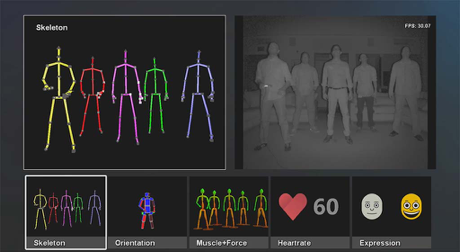
\includegraphics{figures/pic2.png}
        \caption{Kinect v2 detections.}
        \label{fig:fig2}
    \end{figure}

	Given the improvements provided by Microsoft Kinect v2, our experiments were ran on top of it mainly because of higher image quality, reliability and precision regarding face position.
	Another important trait of our project is the integration of Microsoft Kinect with its respective Software Development Kit (SDK) to compute some important values to the developer, as well as the width and height, in pixels, of some object on the screen.
    These values are returned by the methods of \emph{KinectSensor} object, namely \emph{ColorFrameSource} and \emph{DepthFrameSource}.
	Therewith, it is possible to set some regions such as user's head, and retrieve the width, height, and his angle.

	However, for the purpose of this work another class of the SDK Kinect is more important, named \emph{Kinect.Face}. 
	Using this class, it is possible to capture some interesting information, such as: rotation orientation, face engagement, glasses, happy, is left eye closed, is right eye closed, is looking away, has mouth moved, and is mouth open. 
	These values can be seen in Fig. \ref{fig:fig3}, where it is possible to note the information available in the screen provided by the \emph{Kinect.Face} method.

    \begin{figure}[t]
        \centering
        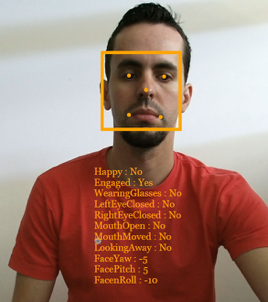
\includegraphics{figures/pic3.png}
        \caption{Information provided by Kinect.Face method.}
        \label{fig:fig3}
    \end{figure}

\section{Eye-Gaze Estimation} \label{sec:eyeGazeEstimation}

\subsection{Predefined Areas}

\subsection{Non-predefined Areas}

\section{Data Extraction} \label{sec:dataExtraction}

\subsection{Clustering}

\section{Conclusion and Future Work} \label{sec:conclusionAndFutureWork}
\todo[inline]{Jean diz: conclusao esta ok tb}
Some clues (such as pointing, gaze and language) are important to make the observer do what is desired. 
In some scenarios, some clues are more important than others, e.g. autism.
Children with autism are known to have difficulties in sharing attention with others, while some researches \cite{14} show that a reasonable proportion of autistic children do not show difficulties in following another's head turn.
Gaze is important to identify what one desires, mainly in cases where one is unable to talk or indicate, e.g. cases of infants and people with disabilities.
Still, in cases such as in Campus work where the gaze was used in a game context and identified that the children tend to avoid confrontation by averting face-directed gazes when they are asking for something, and they gaze longer to attempt to persuade one another.

Our proposal is relevant to aid experiments where there is the need to identify the user gaze in real time and its duration at each region, all given by its head angle.
Moreover, it was possible to create regions of interests according to the length of gazes towards some region, regardless these were predefined or not.
Nevertheless, we identified some problems with the use of this technique solely using head positions. 
One of them is if the head position is slightly tilted to a side, the user could be gazing to the contrary side or the center. 
This can happen because of his iris position. 
Because of that, in this first prototype an image was created from the data of each pixel of the eye region that was informed by the Microsoft Kinect device, showing that the data collected were correct. 

Next, to improve the used technique, k-means clustering was performed to predict the user iris position. 
This algorithm received as input the data which represent the user eye, and then the clusters were created according with similarity of each pixel. 
Based on that, it was possible to perceive that the user iris, depending of the number of clusters, can be easily identified.
As future work, we intend to make the identification of the data that represent the user iris, in an automatic and real time way. 
This would allow a more accurate prediction of user gaze independently of head angle.
\todo[inline]{Again, this is not clear if you used or not the iris positioning}

\begin{figure}[t]
	\centering
	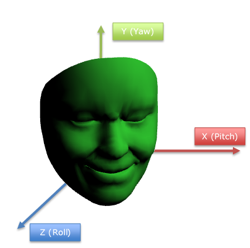
\includegraphics{figures/pic4.png}
    \caption{Quaternions returned by Kinect.Face method and their vertices.}
    \label{fig:fig4}
\end{figure}

\begin{figure}[t]
	\centering
	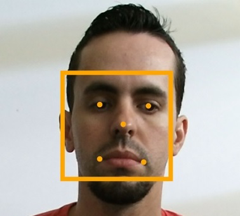
\includegraphics{figures/pic5.png}
    \caption{Predefined face points.}
    \label{fig:fig5}
\end{figure}

\begin{figure}[t]
	\centering
	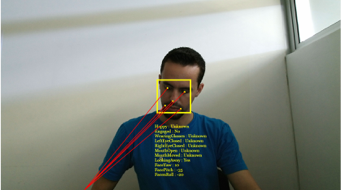
\includegraphics{figures/pic6a.png}\\
    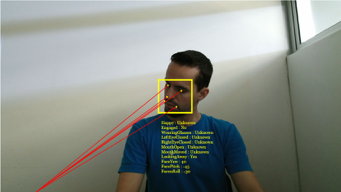
\includegraphics{figures/pic6b.png}\\
    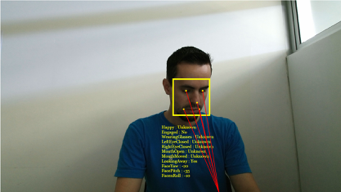
\includegraphics{figures/pic6c.png}\\
	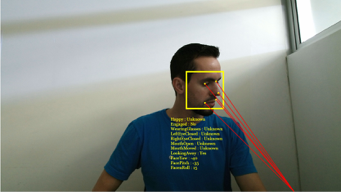
\includegraphics{figures/pic6d.png}
    \caption{Line determined by the head angle and simulating the user gaze.}
    \label{fig:fig6}
\end{figure}

\begin{figure}[t]
	\centering
	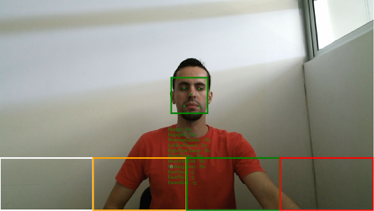
\includegraphics{figures/pic7.png}
    \caption{Regions predefined simulating the cards and other player.}
    \label{fig:fig7}
\end{figure}

\begin{figure}[t]
	\centering
	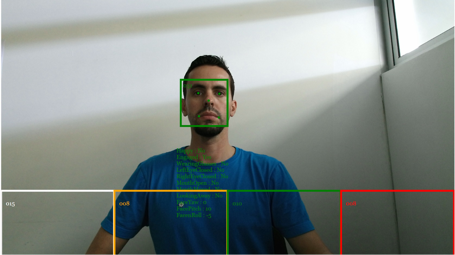
\includegraphics{figures/pic8.png}
    \caption{Seconds observed in each region represented on the left corner of each region.}
    \label{fig:fig8}
\end{figure}

\begin{figure}[t]
	\centering
	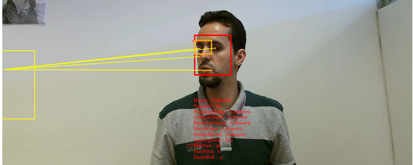
\includegraphics{figures/pic9a.png}\\
    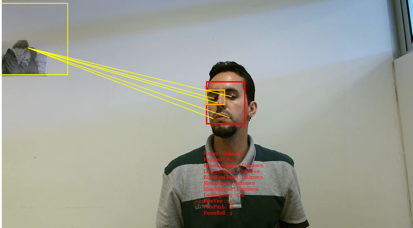
\includegraphics{figures/pic9b.png}\\    
    \caption{Area of interest defined by the system.}
    \label{fig:fig9}
\end{figure}

\begin{figure}[t]
	\centering
	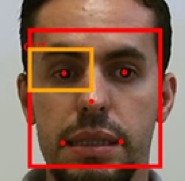
\includegraphics{figures/pic10.png}
    \caption{Eye region identified by the yellow rectangle.}
    \label{fig:fig10}
\end{figure}

\begin{figure}[t]
	\centering
	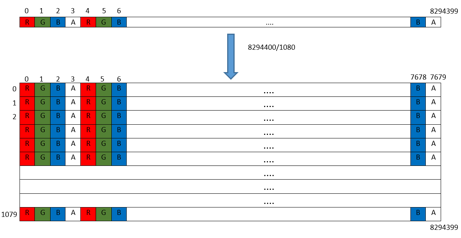
\includegraphics{figures/pic11.png}
    \caption{Representation of color array available by Kinect device.}
    \label{fig:fig11}
\end{figure}

\begin{figure}[t]
	\centering
	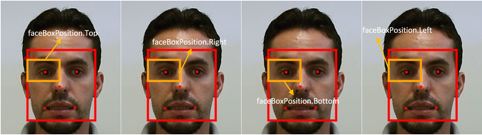
\includegraphics{figures/pic12.png}
    \caption{Indicating the face box position.}
    \label{fig:fig12}
\end{figure}

\begin{figure}[t]
	\centering
	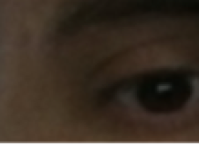
\includegraphics{figures/pic13.png}
    \caption{Image created based on the data in the text file.}
    \label{fig:fig13}
\end{figure}

\begin{figure}[t]
	\centering
	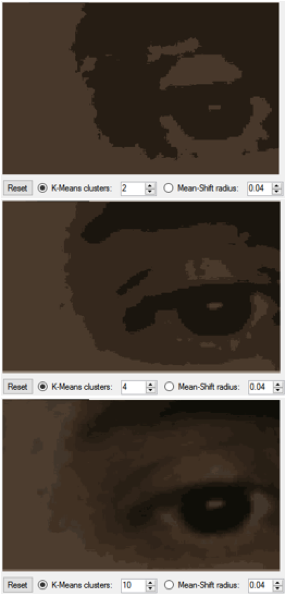
\includegraphics{figures/pic14.png}
    \caption{K-Means test results, at top left was used K = 2, on right K = 3, next, K = 4, K = 5, K = 10 and finally K = 15.}
    \label{fig:fig14}
\end{figure}

\cite{Sibgrapi2016}

\bibliographystyle{IEEEtran}
\bibliography{example}



\end{document}
